\documentclass[12pt]{article}

\usepackage[pdftex]{graphicx}
\usepackage{hyperref}

\hypersetup{colorlinks=true, citecolor=blue, urlcolor=blue}
\usepackage[margin=1in]{geometry}

\usepackage{fancyhdr}
\pagestyle{fancy}

%\usepackage{mathptmx} 
%\linespread{1.05}
%\usepackage[T1]{fontenc}

\setcounter{secnumdepth}{-1} 
\setlength{\headheight}{15pt}

\begin{document}
\fancyhead[LO]{Kaarthik Rajendran and everyone else  \today}



{\Huge 2012 IEEE Region V Robotics Technical Paper}\\[\baselineskip]
{\large\itshape Kaarthik Rajendran }\\[\baselineskip]
\today 

\section{Introduction}
\subsection{Aims}
The challenge was to harvest energy from three different energy sources and deliver to an electrochemical device (i.e. the flag) to measure the amount of energy transmitted. 

\subsection{Objectives}
\begin{itemize}
	\item Capture energy from at least two of three sources (either wind, light, or electric)
	\item Transfer stored energy to the flag mechanism
\end{itemize}
\subsection{Project Restrictions}
\begin{itemize}
	\item The playing field was a 8 foot by 8 foot medium-density fibreboard (MDF) surface divided into four quadrants. Each quadrant consisted of an energy source in the corner. 
\end{itemize}

\begin{figure}[htbp] %  figure placement: here, top, bottom, or page
   \centering
   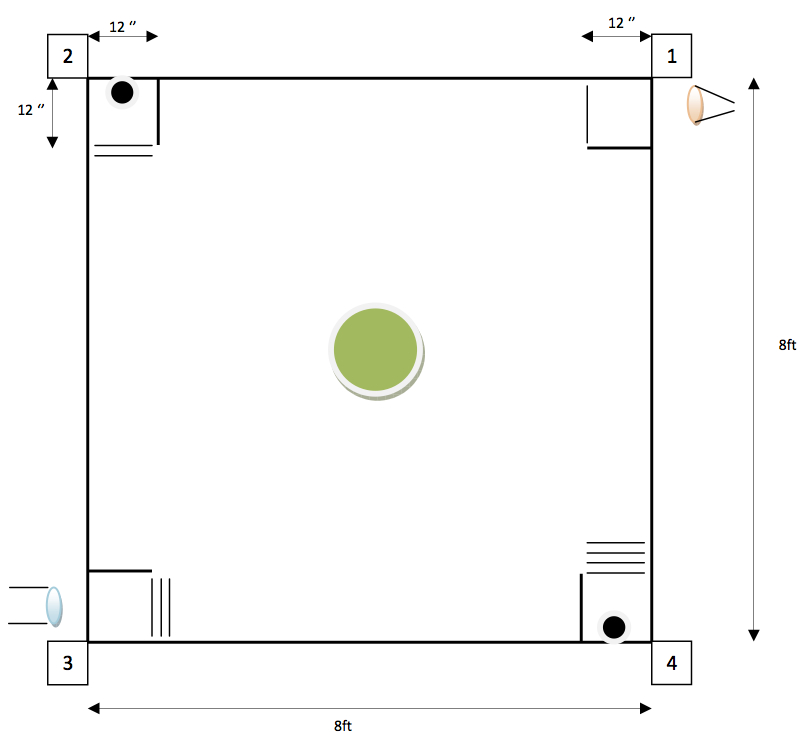
\includegraphics[width=3in]{Robotics2012PlayingField} 
   \caption{example caption}
   \label{fig:example}
\end{figure}

\begin{itemize}
	\item Energy Sources
		\begin{enumerate}
			\item Light Source (Quadrant 1): 50 Watt Halogen MR16 GU10 Base Flood Light Bulb powered by 115 V, 60 Hz Outlet. The center of the bulb was 6 inches above the playing field. The circular surface of the bulb was 6 inches away from the inside surface of the perimeter. 
			\item Electric Source (Quadrant 2): 5 V Thevenin source with 24 Ohm Thevenin resistance. Source is housed in a 3 inch PVC cap. Electrical contacts were 0.5 inch wide thin-metal strips. The top strip was positive. 
			\item Wind Source (Quadrant 3): Style by Revlon 1875 Watt Dryer. Hair Dryer was set on High and Cold Shot permanently depressed. The center of the opening duct was 6 inches above the playing field. The circular surface of the dryer was 6 inches away from the inside surface of the perimeter. 
		\end{enumerate} 
\end{itemize}
\begin{itemize}
	\item Delivery Flag (Quadrant 4): Essentially, a gear motor (Part No. 1094, Pololu Robotics) raises and lowers a small block. TO BE DONE. 
\end{itemize}
\begin{figure}[htbp] %  figure placement: here, top, bottom, or page
   \centering
   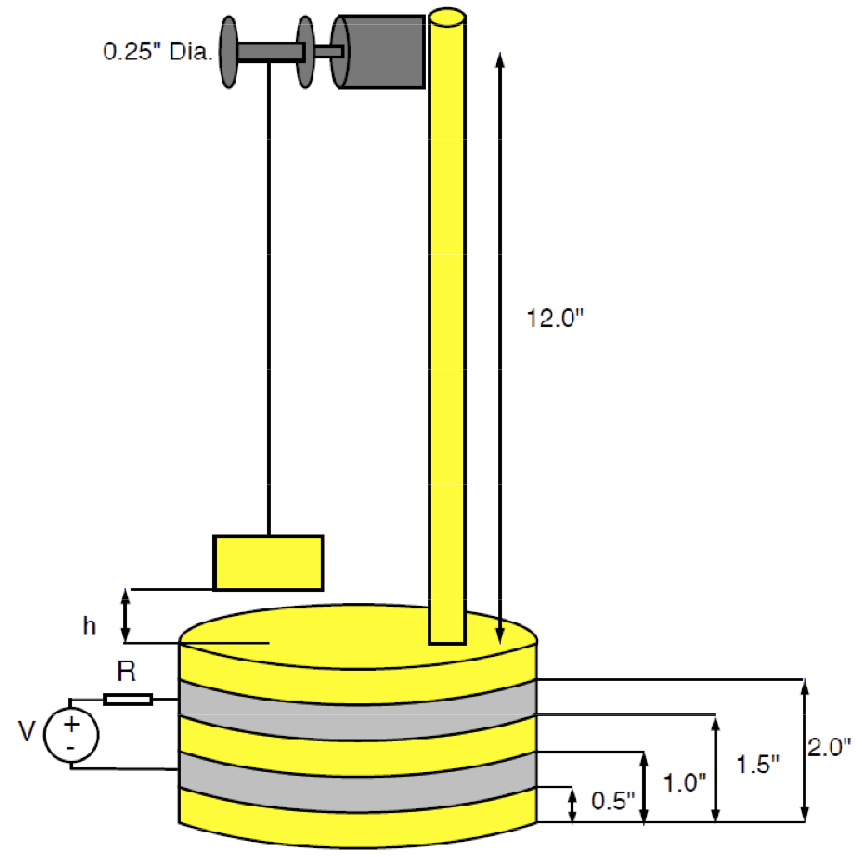
\includegraphics[width=3in]{Robotics2012Flag} 
   \caption{example caption}
   \label{fig:example}
\end{figure}
\begin{itemize}
	\item Starting Tree (Center): TO BE DONE.
	\item Source Switching. TO BE DONE.  
	\item Robot Limitations
		\begin {enumerate}
			\item The robot could not cross the perimeter to harvest light energy or wind energy. 
		\end {enumerate}
\end{itemize}
\end{document}

